\documentclass[12pt]{article}
\usepackage{fontspec}
\usepackage{fullpage}
\usepackage{hyperref}
\hypersetup{bookmarks=true,colorlinks=true,linkcolor=red,citecolor=blue,filecolor=magenta,urlcolor=cyan}
\usepackage{amsmath}
\usepackage{amssymb}
\usepackage{mathtools}
\usepackage{unicode-math}
\usepackage{tabu}
\usepackage{longtable}
\usepackage{booktabs}
\usepackage{caption}
\usepackage{graphics}
\usepackage{enumitem}
\usepackage{filecontents}
\usepackage[backend=bibtex]{biblatex}
\usepackage{url}
\newlist{symbDescription}{description}{1}
\setlist[symbDescription]{noitemsep, topsep=0pt, parsep=0pt, partopsep=0pt}
\setmathfont{Latin Modern Math}
\global\tabulinesep=1mm
\newcounter{assumpnum}
\newcommand{\atheassumpnum}{A\theassumpnum}
\bibliography{bibfile}
\title{Software Requirements Specification for Chipmunk2D}
\author{Alex Halliwushka and Luthfi Mawarid}
\begin{document}
\maketitle
\tableofcontents
\newpage
\section{Reference Material}
\label{Sec:RefMat}
This section records information for easy reference.
\subsection{Table of Units}
\label{Sec:ToU}
The unit system used throughout is SI (Système International d'Unités). In addition to the basic units, several derived units are also used. For each unit, the table lists the symbol, a description and the SI name.
\begin{longtable*}{l l}
\toprule
Symbol & Description
\\
\midrule
kg & mass (kilogram)
\\
m & length (metre)
\\
N & force (newton)
\\
rad & angle (radian)
\\
s & time (second)
\\
\bottomrule
\label{Table:ToU}
\end{longtable*}
\subsection{Table of Symbols}
\label{Sec:ToS}
The table that follows summarizes the symbols used in this document along with their units. Throughout the document, symbols in bold will represent vectors, and scalars otherwise. The symbols are listed in alphabetical order.
\begin{longtabu}{l X[l] l}
\toprule
Symbol & Description & Units
\\
\midrule
$\mathbf{a}$ & Acceleration & $\frac{\text{m}}{\text{s}^{2}}$
\\
${\mathbf{a}_{i}}$ & The I-Th Body's Acceleration & $\frac{\text{m}}{\text{s}^{2}}$
\\
$\mathbf{a}(t)$ & Linear Acceleration & $\frac{\text{m}}{\text{s}^{2}}$
\\
${C_{R}}$ & Coefficient of restitution & --
\\
$\mathbf{F}$ & Force & N
\\
${\mathbf{F}_{1}}$ & Force exerted by the first body (on another body) & N
\\
${\mathbf{F}_{2}}$ & Force exerted by the second body (on another body) & N
\\
${\mathbf{F}_{i}}$ & Force Applied to the I-Th Body at Time T & N
\\
$G$ & Gravitational constant & $\frac{\text{m}^{3}}{(\text{kg}\text{s}^{2})}$
\\
$g$ & Gravitational acceleration & $\frac{\text{m}}{\text{s}^{2}}$
\\
$\mathbf{I}$ & Moment of inertia & kg$\text{m}^{2}$
\\
${\mathbf{I}_{A}}$ & Moment of Inertia Of Rigid Body a & kg$\text{m}^{2}$
\\
${\mathbf{I}_{B}}$ & Moment of Inertia Of Rigid Body B & kg$\text{m}^{2}$
\\
$j$ & Impulse (scalar) & Ns
\\
$L$ & Length & m
\\
$M$ & Total Mass of the Rigid Body & kg
\\
$m$ & Mass & kg
\\
${m_{1}}$ & Mass of the first body & kg
\\
${m_{2}}$ & Mass of the second body & kg
\\
${m_{A}}$ & Mass Of Rigid Body a & kg
\\
${m_{B}}$ & Mass Of Rigid Body B & kg
\\
${m_{j}}$ & Mass Of the J-Th Particle & kg
\\
$\mathbf{n}$ & Collision Normal Vector & m
\\
$\mathbf{p}$ & Position & m
\\
${\mathbf{p}_{CM}}$ & Mass-weighted average position of a rigid body's particles & m
\\
${\mathbf{p}_{j}}$ & Position Vector of the J-Th Particle & m
\\
$\mathbf{r}$ & Displacement & m
\\
${\mathbf{r}_{OB}}$ & Displacement vector between the origin and point B & m
\\
$\mathbf{r}(t)$ & Linear Displacement & m
\\
$\mathbf{\hat{r}}$ & Displacement unit vector & m
\\
$t$ & Time & s
\\
${t_{c}}$ & Denotes the time at collision & s
\\
${{\mathbf{v}_{i}}^{AB}}$ & Relative Velocity Between Rigid Bodies of a and B & $\frac{\text{m}}{\text{s}}$
\\
${\mathbf{v}_{B}}$ & Velocity At Point B & $\frac{\text{m}}{\text{s}}$
\\
${\mathbf{v}_{O}}$ & Velocity At Point Origin & $\frac{\text{m}}{\text{s}}$
\\
$\mathbf{v}$ & Velocity & $\frac{\text{m}}{\text{s}}$
\\
${\mathbf{v}_{A}}$ & Velocity At Point a & $\frac{\text{m}}{\text{s}}$
\\
${\mathbf{v}_{i}}$ & Velocity Of the I-Th Body's Velocity & $\frac{\text{m}}{\text{s}}$
\\
$\mathbf{v}(t)$ & Linear Velocity & $\frac{\text{m}}{\text{s}}$
\\
$||\mathbf{n}||$ & Length of the Normal Vector & m
\\
$||{\mathbf{r}_{AP}}*\mathbf{n}||$ & Length of the Perpendicular Vector To the Contact Displacement Vector of Rigid Body a & m
\\
$||{\mathbf{r}_{BP}}*\mathbf{n}||$ & Length of the Perpendicular Vector To the Contact Displacement Vector of Rigid Body B & m
\\
$||\mathbf{r}||$ & Euclidean norm of the displacement & m
\\
${||\mathbf{r}||^{2}}$ & Squared distance & $\text{m}^{2}$
\\
$α$ & Angular Acceleration & $\frac{\text{rad}}{\text{s}^{2}}$
\\
$θ$ & Angular Displacement & rad
\\
$τ$ & Torque & Nm
\\
${τ_{i}}$ & Torque applied to the i-th body & Nm
\\
$ω$ & Angular Velocity & $\frac{\text{rad}}{\text{s}}$
\\
$ϕ$ & Orientation & rad
\\
\bottomrule
\label{Table:ToS}
\end{longtabu}
\subsection{Abbreviations and Acronyms}
\label{Sec:TAbbAcc}
\begin{longtable*}{l l}
\toprule
Abbreviation & Full Form
\\
\midrule
2D & Two-Dimensional
\\
A & Assumption
\\
CM & Centre of Mass
\\
Chipmunk2D & Chipmunk2D game physics library
\\
DD & Data Definition
\\
GD & General Definition
\\
GS & Goal Statement
\\
IM & Instance Model
\\
LC & Likely Change
\\
ODE & Ordinary Differential Equation
\\
R & Requirement
\\
SRS & Software Requirements Specification
\\
T & Theoretical Model
\\
UC & Unlikely Change
\\
Uncert. & Typical Uncertainty
\\
\bottomrule
\label{Table:TAbbAcc}
\end{longtable*}
\section{Introduction}
\label{Sec:Intro}
Due to the rising cost of developing video games, developers are looking for ways to save time and money for their projects. Using an open source physics library that is reliable and free will cut down development costs and lead to better quality products.
The following section provides an overview of the Software Requirements Specification (SRS) for Chipmunk2D. This section explains the purpose of this document, the scope of the system, the organization of the document, and the characteristics of the intended reader.
\subsection{Purpose of Document}
\label{Sec:DocPurpose}
This document descibes the modeling of an open source 2D rigid body physics library used for games. The theoretical models and goal statements used in Chipmunk2D are provided. This document is intended to be used as a reference to provide all necessary information to understand and verify the model.
This document will be used as a starting point for subsequent development phases, including writing the design specification and the software verification and validation plan. The design document will show how the requirements are to be realized, including decisions on the numerical algorithms and programming environment. The verification and validation plan will show the steps that will be used to increase confidence in the software documentation and the implementation. Although the SRS fits in a series of documents that follow the so-called waterfall model, the actual development process is not constrained in any way. Even when the waterfall model is not followed, as Parnas and Clements point out \cite{parnasClements1986}, the most logical way to present the documentation is still to ``fake'' a rational design process.
\subsection{Scope of Requirements}
\label{Sec:ReqsScope}
The scope of the requirements includes the physical simulation of 2D rigid bodies acted on by forces. Given the appropriate inputs, Chipmunk2D simulates how these rigid bodies interact with one another.
\subsection{Characteristics of Intended Reader}
\label{Sec:ReaderChars}
Reviewers of this documentation should have a strong knowledge in rigid body dynamics. The reviewers should also have an understanding of high school calculus. The users of Chipmunk2D can have a lower level of expertise, as explained in Section~\ref{Sec:UserChars}.
\subsection{Organization of Document}
\label{Sec:DocOrg}
The organization of this document follows the template for an SRS for scientific computing software proposed by \cite{dParnas1972} and \cite{dParnasPcClements1984}. The presentation follows the standard pattern of presenting goals, theories, definitions, and assumptions. For readers that would like a more bottom up approach, they can start reading the instance models in Section~\ref{Sec:IMs} and trace back to find any additional information they require.
The goal statements are refined to the theoretical models, and the theoretical models to the instance models.
\section{General System Description}
\label{Sec:GenSysDesc}
This section provides general information about the system including identifying the interfaces between the system and its environment (system context), describing the user characteristics and listing the system constraints.
\subsection{System Context}
\label{Sec:SysContext}
Figure~\ref{Figure:sysCtxDiag} shows the system context. A circle represents an external entity outside the software, the user in this case. A rectangle represents the software system itself (Chipmunk2D). Arrows are used to show the data flow between the system and its environment.
\begin{figure}
\begin{center}
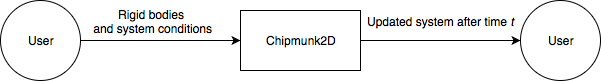
\includegraphics[width=\textwidth]{../../../datafiles/GamePhysics/sysctx.png}
\caption{System Context}
\label{Figure:sysCtxDiag}
\end{center}
\end{figure}
The interaction between the product and the user is through an application programming interface. The responsibilities of the user and the system are as follows:
\begin{itemize}
\item{User Responsibilities}
\begin{itemize}
\item{Provide initial conditions of the physical state of the simulation, rigid bodies present, and forces applied to them.}
\item{Ensure application programming interface use complies with the user guide.}
\item{Ensure required software assumptions (FIXME REF) are appropriate for any particular problem the software addresses.}
\end{itemize}
\item{Chipmunk2D Responsibilities}
\begin{itemize}
\item{Determine if the inputs and simulation state satisfy the required physical and system constraints (FIXME REF).}
\item{Calculate the new state of all rigid bodies within the simulation at each simulation step.}
\item{Provide updated physical state of all rigid bodies at the end of a simulation step.}
\end{itemize}
\end{itemize}
\subsection{User Characteristics}
\label{Sec:UserChars}
The end user of Chipmunk2D should have an understanding of first year programming concepts and an understanding of high school physics.
\subsection{System Constraints}
\label{Sec:SysConstraints}
There are no system constraints.
\section{Specific System Description}
\label{Sec:SpecSystDesc}
This section first presents the problem description, which gives a high-level view of the problem to be solved. This is followed by the solution characteristics specification, which presents the assumptions, theories, and definitions that are used.
\subsection{Problem Description}
\label{Sec:ProbDesc}
Creating a gaming physics library is a difficult task. Games need physics libraries that simulate objects acting under various physical conditions, while simultaneously being fast and efficient enough to work in soft real-time during the game. Developing a physics library from scratch takes a long period of time and is very costly, presenting barriers of entry which make it difficult for game developers to include physics in their products. There are a few free, open source and high quality physics libraries available to be used for consumer products (Section~\ref{Sec:ExistingSolns}). By creating a simple, lightweight, fast and portable 2D rigid body physics library, game development will be more accessible to the masses and higher quality products will be produced.
\subsubsection{Terminology and Definitions}
\label{Sec:TermDefs}
This subsection provides a list of terms that are used in the subsequent sections and their meaning, with the purpose of reducing ambiguity and making it easier to correctly understand the requirements
\begin{itemize}
\item{Rigid body: A solid body in which deformation is neglected.}
\item{Elasticity: Ratio of the relative velocities of two colliding objects after and before a collision.}
\item{Centre of mass: The mean location of the distribution of mass of the object.}
\item{Cartesian coordinate system: A coordinate system that specifies each point uniquely in a plane by a pair of numerical coordinates.}
\item{Right-handed coordinate system: A coordinate system where the positive z-axis comes out of the screen.}
\end{itemize}
\subsubsection{Goal Statements}
\label{Sec:GoalStmt}
Given the inputs, the goal statements are:
\begin{itemize}
\item[GS1:]Given the physical properties, initial positions and velocities, and forces applied on a set of rigid bodies, determine their new positions and velocities over a period of time.
\item[GS2:]Given the physical properties, initial orientations and angular velocities, and forces applied on a set of rigid bodies, determine their new orientations and angular velocities over a period of time.
\item[GS3:]Given the initial positions and velocities of a set of rigid bodies, determine if any of them will collide with one another over a period of time.
\item[GS4:]Given the physical properties, initial positions, orientations, linear velocities, and angular velocities of a set of rigid bodies, determine the new positions, orientations, linear velocities, and angular velocities over a period of time of the rigid bodies that have undergone a collision.
\end{itemize}
\subsection{Solution Characteristics Specification}
\label{Sec:SolCharSpec}
The instance models that govern Chipmunk2D are presented in Section~\ref{Sec:IMs}. The information to understand the meaning of the instance models and their derivation is also presented, so that the instance models can be verified.
\subsubsection{Assumptions}
\label{Sec:Assumps}
This section simplifies the original problem and helps in developing the theoretical model by filling in the missing information for the physical system. The numbers given in the square brackets refer to the Theoretical Models {[}Section~\ref{Sec:TMs}{]}, General Definitions {[}Section~\ref{Sec:GDs}{]}, Data Definitions {[}Section~\ref{Sec:DDs}{]}, Instance Models {[}Section~\ref{Sec:IMs}{]}, Likely Changes {[}Section~\ref{Sec:LCs}{]}, or Unlikely Changes {[}Section~\ref{Sec:UCs}{]}, in which the respective assumption is used.
\begin{description}
\item[\refstepcounter{assumpnum}\atheassumpnum\label{A:objectTy}:]All objects are rigid bodies.
\end{description}
\begin{description}
\item[\refstepcounter{assumpnum}\atheassumpnum\label{A:objectDimension}:]All objects are 2D.
\end{description}
\begin{description}
\item[\refstepcounter{assumpnum}\atheassumpnum\label{A:coordinateSystemTy}:]The library uses a Cartesian coordinate system.
\end{description}
\begin{description}
\item[\refstepcounter{assumpnum}\atheassumpnum\label{A:axesDefined}:]The axes are defined using right-handed coordinate system.
\end{description}
\begin{description}
\item[\refstepcounter{assumpnum}\atheassumpnum\label{A:collisionType}:]All rigid bodies collisions are vertex-to-edge collisions.
\end{description}
\begin{description}
\item[\refstepcounter{assumpnum}\atheassumpnum\label{A:dampingInvolvement}:]There is no damping involved throughout the simulation.
\end{description}
\begin{description}
\item[\refstepcounter{assumpnum}\atheassumpnum\label{A:constraintsAndJointsInvolvement}:]There are no constraints and joints involved throughout the simulation.
\end{description}
\subsubsection{Theoretical Models}
\label{Sec:TMs}
This section focuses on the general equations and laws that Chipmunk2D is based on.
~\newline
\noindent \begin{minipage}{\textwidth}
\begin{tabular}{p{0.2\textwidth} p{0.73\textwidth}}
\toprule \textbf{Refname} & \textbf{T:newtonSL}
\phantomsection 
\label{T:newtonSL}
\\ \midrule \\
Label & Newton's second law of motion
\\ \midrule \\
Equation & \begin{dmath}
           \mathbf{F}=m \mathbf{a}
           \end{dmath}
\\ \midrule \\
Description & \begin{symbDescription}
              \item{$\mathbf{F}$ is the force (N)}
              \item{$m$ is the mass (kg)}
              \item{$\mathbf{a}$ is the acceleration ($\frac{\text{m}}{\text{s}^{2}}$)}
              \end{symbDescription}
\\ \midrule \\
Notes & The net force $\mathbf{F}$ (N) on a rigid body is proportional to the acceleration $\mathbf{a}$ ($\frac{\text{m}}{\text{s}^{2}}$) of the rigid body, where $m$ (kg) denotes the mass of the rigid body as the constant of proportionality.
\\ \midrule \\
Source & 
\\ \midrule \\
RefBy & FIXME: This needs to be filled in
\\ \bottomrule \end{tabular}
\end{minipage}\\
~\newline
\noindent \begin{minipage}{\textwidth}
\begin{tabular}{p{0.2\textwidth} p{0.73\textwidth}}
\toprule \textbf{Refname} & \textbf{T:newtonTL}
\phantomsection 
\label{T:newtonTL}
\\ \midrule \\
Label & Newton's third law of motion
\\ \midrule \\
Equation & \begin{dmath}
           {\mathbf{F}_{1}}=-{\mathbf{F}_{2}}
           \end{dmath}
\\ \midrule \\
Description & \begin{symbDescription}
              \item{${\mathbf{F}_{1}}$ is the force exerted by the first body (on another body) (N)}
              \item{${\mathbf{F}_{2}}$ is the force exerted by the second body (on another body) (N)}
              \end{symbDescription}
\\ \midrule \\
Notes & Every action has an equal and opposite reaction. In other words, the force ${\mathbf{F}_{1}}$ (N) exerted on the second rigid body by the first is equal in magnitude and in the opposite direction to the force ${\mathbf{F}_{2}}$ (N) exerted on the first rigid body by the second.
\\ \midrule \\
Source & 
\\ \midrule \\
RefBy & FIXME: This needs to be filled in
\\ \bottomrule \end{tabular}
\end{minipage}\\
~\newline
\noindent \begin{minipage}{\textwidth}
\begin{tabular}{p{0.2\textwidth} p{0.73\textwidth}}
\toprule \textbf{Refname} & \textbf{T:newtonLUG}
\phantomsection 
\label{T:newtonLUG}
\\ \midrule \\
Label & Newton's law of universal gravitation
\\ \midrule \\
Equation & \begin{dmath}
           \mathbf{F}=G \frac{{m_{1}} {m_{2}}}{||\mathbf{r}||^{2}} \mathbf{\hat{r}}=G \frac{{m_{1}} {m_{2}}}{||\mathbf{r}||^{2}} \frac{\mathbf{r}}{||\mathbf{r}||}
           \end{dmath}
\\ \midrule \\
Description & \begin{symbDescription}
              \item{$\mathbf{F}$ is the force (N)}
              \item{$G$ is the gravitational constant ($\frac{\text{m}^{3}}{(\text{kg}\text{s}^{2})}$)}
              \item{${m_{1}}$ is the mass of the first body (kg)}
              \item{${m_{2}}$ is the mass of the second body (kg)}
              \item{$||\mathbf{r}||$ is the Euclidean norm of the displacement (m)}
              \item{$\mathbf{\hat{r}}$ is the displacement unit vector (m)}
              \item{$\mathbf{r}$ is the displacement (m)}
              \end{symbDescription}
\\ \midrule \\
Notes & Two rigid bodies in the universe attract each other with a force $\mathbf{F}$ (N) that is directly proportional to the product of their masses, ${m_{1}}$ and ${m_{2}}$ (kg), and inversely proportional to the squared distance ${||\mathbf{r}||^{2}}$ ($\text{m}^{2}$) between them. The vector $\mathbf{r}$ (m) is the displacement between the centres of the rigid bodies and $||\mathbf{r}||$ (m) represents the Euclidean norm of the displacement, or absolute distance between the two. $\mathbf{\hat{r}}$ denotes the displacement unit vector, equivalent to the displacement divided by the Euclidean norm of the displacement, as shown above. Finally, $G$ is the gravitational constant (6.673 * 10E-11) ($\frac{\text{m}^{3}}{(\text{kg}\text{s}^{2})}$).
\\ \midrule \\
Source & 
\\ \midrule \\
RefBy & FIXME: This needs to be filled in
\\ \bottomrule \end{tabular}
\end{minipage}\\
~\newline
\noindent \begin{minipage}{\textwidth}
\begin{tabular}{p{0.2\textwidth} p{0.73\textwidth}}
\toprule \textbf{Refname} & \textbf{T:chaslesThm}
\phantomsection 
\label{T:chaslesThm}
\\ \midrule \\
Label & Chasles' theorem
\\ \midrule \\
Equation & \begin{dmath}
           {\mathbf{v}_{B}}={\mathbf{v}_{O}}+ω\times{\mathbf{r}_{OB}}
           \end{dmath}
\\ \midrule \\
Description & \begin{symbDescription}
              \item{${\mathbf{v}_{B}}$ is the velocity at point B ($\frac{\text{m}}{\text{s}}$)}
              \item{${\mathbf{v}_{O}}$ is the velocity at point origin ($\frac{\text{m}}{\text{s}}$)}
              \item{$ω$ is the angular velocity ($\frac{\text{rad}}{\text{s}}$)}
              \item{${\mathbf{r}_{OB}}$ is the displacement vector between the origin and point B (m)}
              \end{symbDescription}
\\ \midrule \\
Notes & The linear velocity ${\mathbf{v}_{B}}$ ($\frac{\text{m}}{\text{s}}$) of any point B in a rigid body is the sum of the linear velocity ${\mathbf{v}_{O}}$ ($\frac{\text{m}}{\text{s}}$) of the rigid body at the origin (axis of rotation) and the resultant vector from the cross product of the rigid body's angular velocity $ω$ ($\frac{\text{rad}}{\text{s}}$) and the displacement vector between the origin and point B, ${\mathbf{r}_{OB}}$ (m).
\\ \midrule \\
Source & 
\\ \midrule \\
RefBy & FIXME: This needs to be filled in
\\ \bottomrule \end{tabular}
\end{minipage}\\
~\newline
\noindent \begin{minipage}{\textwidth}
\begin{tabular}{p{0.2\textwidth} p{0.73\textwidth}}
\toprule \textbf{Refname} & \textbf{T:newtonSLR}
\phantomsection 
\label{T:newtonSLR}
\\ \midrule \\
Label & Newton's second law for rotational motion
\\ \midrule \\
Equation & \begin{dmath}
           τ=\mathbf{I} α
           \end{dmath}
\\ \midrule \\
Description & \begin{symbDescription}
              \item{$τ$ is the torque (Nm)}
              \item{$\mathbf{I}$ is the moment of inertia (kg$\text{m}^{2}$)}
              \item{$α$ is the angular acceleration ($\frac{\text{rad}}{\text{s}^{2}}$)}
              \end{symbDescription}
\\ \midrule \\
Notes & The net torque $τ$ (Nm) on a rigid body is proportional to its angular acceleration $α$ ($\frac{\text{rad}}{\text{s}^{2}}$). Here, $\mathbf{I}$ (kg$\text{m}^{2}$) denotes the moment of inertia of the rigid body. We also assume that all rigid bodies involved are two-dimensional (A2).
\\ \midrule \\
Source & 
\\ \midrule \\
RefBy & FIXME: This needs to be filled in
\\ \bottomrule \end{tabular}
\end{minipage}\\
\subsubsection{General Definitions}
\label{Sec:GDs}
There are no general definitions.
\subsubsection{Instance Models}
\label{Sec:IMs}
This section transforms the problem defined in Section~\ref{Sec:ProbDesc} into one which is expressed in mathematical terms. It uses concrete symbols defined in Section~\ref{Sec:DDs} to replace the abstract symbols in the models identified in Section~\ref{Sec:TMs} and Section~\ref{Sec:GDs}.
~\newline
\noindent \begin{minipage}{\textwidth}
\begin{tabular}{p{0.2\textwidth} p{0.73\textwidth}}
\toprule \textbf{Refname} & \textbf{IM:transMot}
\phantomsection 
\label{IM:transMot}
\\ \midrule \\
Label & Force on the translational motion of a set of 2d rigid bodies
\\ \midrule \\
Input & ${\mathbf{v}_{i}}$, $t$, $g$, ${\mathbf{F}_{i}}$, ${m_{j}}$
\\ \midrule \\
Output & ${\mathbf{a}_{i}}$
\\ \midrule \\
Input Constraints & \begin{dmath}
                    {\mathbf{v}_{i}}>0
                    \end{dmath}
                    \begin{dmath}
                    t>0
                    \end{dmath}
                    \begin{dmath}
                    g>0
                    \end{dmath}
                    \begin{dmath}
                    {\mathbf{F}_{i}}>0
                    \end{dmath}
                    \begin{dmath}
                    {m_{j}}>0
                    \end{dmath}
\\ \midrule \\
Output Constraints & 
\\ \midrule \\
Equation & \begin{dmath}
           {\mathbf{a}_{i}}=\frac{d\,{\mathbf{v}_{i}}\left(t\right)}{d\,t}=g+\frac{{\mathbf{F}_{i}}\left(t\right)}{{m_{j}}}
           \end{dmath}
\\ \midrule \\
Description & \begin{symbDescription}
              \item{${\mathbf{a}_{i}}$ is the the i-th body's acceleration ($\frac{\text{m}}{\text{s}^{2}}$)}
              \item{$t$ is the time (s)}
              \item{${\mathbf{v}_{i}}$ is the velocity of the i-th body's velocity ($\frac{\text{m}}{\text{s}}$)}
              \item{$g$ is the gravitational acceleration ($\frac{\text{m}}{\text{s}^{2}}$)}
              \item{${\mathbf{F}_{i}}$ is the force applied to the i-th body at time t (N)}
              \item{${m_{j}}$ is the mass of the j-th particle (kg)}
              \end{symbDescription}
\\ \midrule \\
Notes & The above equation expresses the total acceleration of the rigid body (A1, A2) i as the sum of gravitational acceleration (GD3) and acceleration due to applied force Fi(t) (T1). The resultant outputs are then obtained from this equation using DD2, DD3 and DD4. It is currently assumed that there is no damping (A6) or constraints (A7) involved.
\\ \midrule \\
Source & 
\\ \midrule \\
RefBy & FIXME: This needs to be filled in
\\ \bottomrule \end{tabular}
\end{minipage}\\
~\newline
\noindent \begin{minipage}{\textwidth}
\begin{tabular}{p{0.2\textwidth} p{0.73\textwidth}}
\toprule \textbf{Refname} & \textbf{IM:rotMot}
\phantomsection 
\label{IM:rotMot}
\\ \midrule \\
Label & Force on the rotational motion of a set of 2D rigid body
\\ \midrule \\
Input & $ω$, $t$, ${τ_{i}}$, $\mathbf{I}$
\\ \midrule \\
Output & $α$
\\ \midrule \\
Input Constraints & \begin{dmath}
                    ω>0
                    \end{dmath}
                    \begin{dmath}
                    t>0
                    \end{dmath}
                    \begin{dmath}
                    {τ_{i}}>0
                    \end{dmath}
                    \begin{dmath}
                    \mathbf{I}>0
                    \end{dmath}
\\ \midrule \\
Output Constraints & \begin{dmath}
                     α>0
                     \end{dmath}
\\ \midrule \\
Equation & \begin{dmath}
           α=\frac{d\,ω\left(t\right)}{d\,t}=\frac{{τ_{i}}\left(t\right)}{\mathbf{I}}
           \end{dmath}
\\ \midrule \\
Description & \begin{symbDescription}
              \item{$α$ is the angular acceleration ($\frac{\text{rad}}{\text{s}^{2}}$)}
              \item{$t$ is the time (s)}
              \item{$ω$ is the angular velocity ($\frac{\text{rad}}{\text{s}}$)}
              \item{${τ_{i}}$ is the torque applied to the i-th body (Nm)}
              \item{$\mathbf{I}$ is the moment of inertia (kg$\text{m}^{2}$)}
              \end{symbDescription}
\\ \midrule \\
Notes & The above equation for the total angular acceleration of the rigid body (A1, A2) i is derived from T5, and the resultant outputs are then obtained from this equation using DD5, DD6 and DD7. It is currently assumed that there is no damping (A6) or constraints (A7) involved.
\\ \midrule \\
Source & 
\\ \midrule \\
RefBy & FIXME: This needs to be filled in
\\ \bottomrule \end{tabular}
\end{minipage}\\
~\newline
\noindent \begin{minipage}{\textwidth}
\begin{tabular}{p{0.2\textwidth} p{0.73\textwidth}}
\toprule \textbf{Refname} & \textbf{IM:col2D}
\phantomsection 
\label{IM:col2D}
\\ \midrule \\
Label & Collisions on 2D rigid bodies
\\ \midrule \\
Input & $t$, $j$, ${m_{A}}$, $\mathbf{n}$
\\ \midrule \\
Output & ${t_{c}}$
\\ \midrule \\
Input Constraints & \begin{dmath}
                    t>0
                    \end{dmath}
                    \begin{dmath}
                    j>0
                    \end{dmath}
                    \begin{dmath}
                    {m_{A}}>0
                    \end{dmath}
                    \begin{dmath}
                    \mathbf{n}>0
                    \end{dmath}
\\ \midrule \\
Output Constraints & \begin{dmath}
                     {\mathbf{v}_{A}}>0
                     \end{dmath}
                     \begin{dmath}
                     {t_{c}}>0
                     \end{dmath}
\\ \midrule \\
Equation & \begin{dmath}
           {\mathbf{v}_{A}}\left({t_{c}}\right)={\mathbf{v}_{A}}\left(t\right)+\frac{j}{{m_{A}}} \mathbf{n}
           \end{dmath}
\\ \midrule \\
Description & \begin{symbDescription}
              \item{${\mathbf{v}_{A}}$ is the velocity at point A ($\frac{\text{m}}{\text{s}}$)}
              \item{${t_{c}}$ is the denotes the time at collision (s)}
              \item{$t$ is the time (s)}
              \item{$j$ is the impulse (scalar) (Ns)}
              \item{${m_{A}}$ is the mass of rigid body A (kg)}
              \item{$\mathbf{n}$ is the collision normal vector (m)}
              \end{symbDescription}
\\ \midrule \\
Notes & This instance model is based on our assumptions regarding rigid body (A1, A2) collisions (A5). Again, this does not take damping (A6) or constraints (A7) into account.
\\ \midrule \\
Source & 
\\ \midrule \\
RefBy & FIXME: This needs to be filled in
\\ \bottomrule \end{tabular}
\end{minipage}\\
\subsubsection{Data Definitions}
\label{Sec:DDs}
This section collects and defines all the data needed to build the instance models.
~\newline
\noindent \begin{minipage}{\textwidth}
\begin{tabular}{p{0.2\textwidth} p{0.73\textwidth}}
\toprule \textbf{Refname} & \textbf{DD:ctrOfMass}
\phantomsection 
\label{DD:ctrOfMass}
\\ \midrule \\
Label & Mass-weighted average position of a rigid body's particles
\\ \midrule \\
Symbol & ${\mathbf{p}_{CM}}$
\\ \midrule \\
Units & m
\\ \midrule \\
Equation & \begin{dmath}
           {\mathbf{p}_{CM}}=\frac{\displaystyle\sum{{m_{j}} {\mathbf{p}_{j}}}}{M}
           \end{dmath}
\\ \midrule \\
Description & \begin{symbDescription}
              \item{${\mathbf{p}_{CM}}$ is the mass-weighted average position of a rigid body's particles (m)}
              \item{${m_{j}}$ is the mass of the j-th particle (kg)}
              \item{${\mathbf{p}_{j}}$ is the position vector of the j-th particle (m)}
              \item{$M$ is the total mass of the rigid body (kg)}
              \end{symbDescription}
\\ \midrule \\
Source & 
\\ \midrule \\
RefBy & FIXME: This needs to be filled in
\\ \bottomrule \end{tabular}
\end{minipage}\\
~\newline
\noindent \begin{minipage}{\textwidth}
\begin{tabular}{p{0.2\textwidth} p{0.73\textwidth}}
\toprule \textbf{Refname} & \textbf{DD:linDisp}
\phantomsection 
\label{DD:linDisp}
\\ \midrule \\
Label & Linear Displacement
\\ \midrule \\
Symbol & $\mathbf{r}(t)$
\\ \midrule \\
Units & m
\\ \midrule \\
Equation & \begin{dmath}
           \mathbf{r}(t)=\frac{d\,\mathbf{p}\left(t\right)}{d\,t}
           \end{dmath}
\\ \midrule \\
Description & \begin{symbDescription}
              \item{$\mathbf{r}(t)$ is the linear displacement (m)}
              \item{$t$ is the time (s)}
              \item{$\mathbf{p}$ is the position (m)}
              \end{symbDescription}
\\ \midrule \\
Source & 
\\ \midrule \\
RefBy & FIXME: This needs to be filled in
\\ \bottomrule \end{tabular}
\end{minipage}\\
~\newline
\noindent \begin{minipage}{\textwidth}
\begin{tabular}{p{0.2\textwidth} p{0.73\textwidth}}
\toprule \textbf{Refname} & \textbf{DD:linVel}
\phantomsection 
\label{DD:linVel}
\\ \midrule \\
Label & Linear Velocity
\\ \midrule \\
Symbol & $\mathbf{v}(t)$
\\ \midrule \\
Units & $\frac{\text{m}}{\text{s}}$
\\ \midrule \\
Equation & \begin{dmath}
           \mathbf{v}(t)=\frac{d\,\mathbf{r}\left(t\right)}{d\,t}
           \end{dmath}
\\ \midrule \\
Description & \begin{symbDescription}
              \item{$\mathbf{v}(t)$ is the linear velocity ($\frac{\text{m}}{\text{s}}$)}
              \item{$t$ is the time (s)}
              \item{$\mathbf{r}$ is the displacement (m)}
              \end{symbDescription}
\\ \midrule \\
Source & 
\\ \midrule \\
RefBy & FIXME: This needs to be filled in
\\ \bottomrule \end{tabular}
\end{minipage}\\
~\newline
\noindent \begin{minipage}{\textwidth}
\begin{tabular}{p{0.2\textwidth} p{0.73\textwidth}}
\toprule \textbf{Refname} & \textbf{DD:linAcc}
\phantomsection 
\label{DD:linAcc}
\\ \midrule \\
Label & Linear Acceleration
\\ \midrule \\
Symbol & $\mathbf{a}(t)$
\\ \midrule \\
Units & $\frac{\text{m}}{\text{s}^{2}}$
\\ \midrule \\
Equation & \begin{dmath}
           \mathbf{a}(t)=\frac{d\,\mathbf{v}\left(t\right)}{d\,t}
           \end{dmath}
\\ \midrule \\
Description & \begin{symbDescription}
              \item{$\mathbf{a}(t)$ is the linear acceleration ($\frac{\text{m}}{\text{s}^{2}}$)}
              \item{$t$ is the time (s)}
              \item{$\mathbf{v}$ is the velocity ($\frac{\text{m}}{\text{s}}$)}
              \end{symbDescription}
\\ \midrule \\
Source & 
\\ \midrule \\
RefBy & FIXME: This needs to be filled in
\\ \bottomrule \end{tabular}
\end{minipage}\\
~\newline
\noindent \begin{minipage}{\textwidth}
\begin{tabular}{p{0.2\textwidth} p{0.73\textwidth}}
\toprule \textbf{Refname} & \textbf{DD:angDisp}
\phantomsection 
\label{DD:angDisp}
\\ \midrule \\
Label & Angular Displacement
\\ \midrule \\
Symbol & $θ$
\\ \midrule \\
Units & rad
\\ \midrule \\
Equation & \begin{dmath}
           θ=\frac{d\,ϕ\left(t\right)}{d\,t}
           \end{dmath}
\\ \midrule \\
Description & \begin{symbDescription}
              \item{$θ$ is the angular displacement (rad)}
              \item{$t$ is the time (s)}
              \item{$ϕ$ is the orientation (rad)}
              \end{symbDescription}
\\ \midrule \\
Source & 
\\ \midrule \\
RefBy & FIXME: This needs to be filled in
\\ \bottomrule \end{tabular}
\end{minipage}\\
~\newline
\noindent \begin{minipage}{\textwidth}
\begin{tabular}{p{0.2\textwidth} p{0.73\textwidth}}
\toprule \textbf{Refname} & \textbf{DD:angVel}
\phantomsection 
\label{DD:angVel}
\\ \midrule \\
Label & Angular Velocity
\\ \midrule \\
Symbol & $ω$
\\ \midrule \\
Units & $\frac{\text{rad}}{\text{s}}$
\\ \midrule \\
Equation & \begin{dmath}
           ω=\frac{d\,θ\left(t\right)}{d\,t}
           \end{dmath}
\\ \midrule \\
Description & \begin{symbDescription}
              \item{$ω$ is the angular velocity ($\frac{\text{rad}}{\text{s}}$)}
              \item{$t$ is the time (s)}
              \item{$θ$ is the angular displacement (rad)}
              \end{symbDescription}
\\ \midrule \\
Source & 
\\ \midrule \\
RefBy & FIXME: This needs to be filled in
\\ \bottomrule \end{tabular}
\end{minipage}\\
~\newline
\noindent \begin{minipage}{\textwidth}
\begin{tabular}{p{0.2\textwidth} p{0.73\textwidth}}
\toprule \textbf{Refname} & \textbf{DD:angAccel}
\phantomsection 
\label{DD:angAccel}
\\ \midrule \\
Label & Angular Acceleration
\\ \midrule \\
Symbol & $α$
\\ \midrule \\
Units & $\frac{\text{rad}}{\text{s}^{2}}$
\\ \midrule \\
Equation & \begin{dmath}
           α=\frac{d\,ω\left(t\right)}{d\,t}
           \end{dmath}
\\ \midrule \\
Description & \begin{symbDescription}
              \item{$α$ is the angular acceleration ($\frac{\text{rad}}{\text{s}^{2}}$)}
              \item{$t$ is the time (s)}
              \item{$ω$ is the angular velocity ($\frac{\text{rad}}{\text{s}}$)}
              \end{symbDescription}
\\ \midrule \\
Source & 
\\ \midrule \\
RefBy & FIXME: This needs to be filled in
\\ \bottomrule \end{tabular}
\end{minipage}\\
~\newline
\noindent \begin{minipage}{\textwidth}
\begin{tabular}{p{0.2\textwidth} p{0.73\textwidth}}
\toprule \textbf{Refname} & \textbf{DD:impulse}
\phantomsection 
\label{DD:impulse}
\\ \midrule \\
Label & Impulse (scalar)
\\ \midrule \\
Symbol & $j$
\\ \midrule \\
Units & Ns
\\ \midrule \\
Equation & \begin{dmath}
           j=\frac{-\left(1+{C_{R}}\right) {{\mathbf{v}_{i}}^{AB}}\cdot{}\mathbf{n}}{\left(\frac{1}{{m_{A}}}+\frac{1}{{m_{B}}}\right) ||\mathbf{n}||^{2}+\frac{||{\mathbf{r}_{AP}}*\mathbf{n}||^{2}}{{\mathbf{I}_{A}}}+\frac{||{\mathbf{r}_{BP}}*\mathbf{n}||^{2}}{{\mathbf{I}_{B}}}}
           \end{dmath}
\\ \midrule \\
Description & \begin{symbDescription}
              \item{$j$ is the impulse (scalar) (Ns)}
              \item{${C_{R}}$ is the coefficient of restitution (Unitless)}
              \item{${{\mathbf{v}_{i}}^{AB}}$ is the relative velocity between rigid bodies of A and B ($\frac{\text{m}}{\text{s}}$)}
              \item{$\mathbf{n}$ is the collision normal vector (m)}
              \item{${m_{A}}$ is the mass of rigid body A (kg)}
              \item{${m_{B}}$ is the mass of rigid body B (kg)}
              \item{$||\mathbf{n}||$ is the length of the normal vector (m)}
              \item{$||{\mathbf{r}_{AP}}*\mathbf{n}||$ is the length of the perpendicular vector to the contact displacement vector of rigid body A (m)}
              \item{${\mathbf{I}_{A}}$ is the moment of inertia of rigid body A (kg$\text{m}^{2}$)}
              \item{$||{\mathbf{r}_{BP}}*\mathbf{n}||$ is the length of the perpendicular vector to the contact displacement vector of rigid body B (m)}
              \item{${\mathbf{I}_{B}}$ is the moment of inertia of rigid body B (kg$\text{m}^{2}$)}
              \end{symbDescription}
\\ \midrule \\
Source & 
\\ \midrule \\
RefBy & FIXME: This needs to be filled in
\\ \bottomrule \end{tabular}
\end{minipage}\\
\subsubsection{Data Constraints}
\label{Sec:DataConstraints}
Table~\ref{Table:InDataConstraints} and Table~\ref{Table:OutDataConstraints} show the data constraints on the input and output variables, respectively. The column for physical constraints gives the physical limitations on the range of values that can be taken by the variable. The uncertainty column provides an estimate of the confidence with which the physical quantities can be measured. This information would be part of the input if one were performing an uncertainty quantification exercise. The constraints are conservative, to give the user of the model the flexibility to experiment with unusual situations. The column of typical values is intended to provide a feel for a common scenario. FIXME
\begin{longtable}{l l l l}
\toprule
Var & Physical Constraints & Typical Value & Uncert.
\\
\midrule
${C_{R}}$ & $0\leq{}{C_{R}}\leq{}1$ & $800.0\cdot{}10^{-3}$ & 10.0\%
\\
$\mathbf{F}$ & -- & $98.1$ N & 10.0\%
\\
$G$ & -- & $9.8$ $\frac{\text{m}^{3}}{(\text{kg}\text{s}^{2})}$ & 10.0\%
\\
$\mathbf{I}$ & $\mathbf{I}\geq{}0$ & $74.5$ kg$\text{m}^{2}$ & 10.0\%
\\
$L$ & $L\geq{}0$ & $44.2$ m & 10.0\%
\\
$m$ & $m\geq{}0$ & $56.2$ kg & 10.0\%
\\
$\mathbf{p}$ & -- & $412.0\cdot{}10^{-3}$ m & 10.0\%
\\
$\mathbf{v}$ & -- & $2.51$ $\frac{\text{m}}{\text{s}}$ & 10.0\%
\\
$τ$ & -- & $200.0$ Nm & 10.0\%
\\
$ω$ & -- & $2.1$ $\frac{\text{rad}}{\text{s}}$ & 10.0\%
\\
$ϕ$ & -- & $\frac{π}{2}$ rad & 10.0\%
\\
\bottomrule
\caption{Input Data Constraints}
\label{Table:InDataConstraints}
\end{longtable}
\begin{longtable}{l}
\toprule
Var
\\
\midrule
$\mathbf{p}$
\\
$\mathbf{v}$
\\
$ϕ$
\\
$ω$
\\
\bottomrule
\caption{Output Data Constraints}
\label{Table:OutDataConstraints}
\end{longtable}
\section{Requirements}
\label{Sec:Requirements}
This section provides the functional requirements, the business tasks that the software is expected to complete, and the non-functional requirements, the qualities that the software is expected to exhibit.
\subsection{Functional Requirements}
\label{Sec:FRs}
\begin{itemize}
\item[R1:]Create a space for all of the rigid bodies in the physical simulation to interact in.
\item[R2:]Input the initial masses, velocities, orientations, angular velocities of, and forces applied on rigid bodies.
\item[R3:]Input the surface properties of the bodies such as friction or elasticity.
\item[R4:]Verify that the inputs satisfy the required physical constraints from Section~\ref{Sec:SolCharSpec}.
\item[R5:]Determine the positions and velocities over a period of time of the 2D rigid bodies acted upon by a force.
\item[R6:]Determine the orientations and angular velocities over a period of time of the 2D rigid bodies.
\item[R7:]Determine if any of the rigid bodies in the space have collided.
\item[R8:]Determine the positions and velocities over a period of time of the 2D rigid bodies that have undergone a collision.
\end{itemize}
\subsection{Non-Functional Requirements}
\label{Sec:NFRs}
Games are resource intensive, so performance is a high priority. Other non-functional requirements that are a priority are: correctness, understandability, portability, reliability, and maintainability.
\section{Likely Changes}
\label{Sec:LCs}
This section lists the likely changes to be made to the game physics library.
\begin{itemize}
\item[LC1:]The internal ODE-solving algorithm used by the library may be changed in the future.
\item[LC2:]The library may be expanded to deal with edge-to-edge and vertex-to-vertex collisions.
\item[LC3:]The library may be expanded to include motion with damping.
\item[LC4:]The library may be expanded to include joints and constraints.
\end{itemize}
\section{Unlikely Changes}
\label{Sec:UCs}
This section lists the unlikely changes to be made to the game physics library.
\begin{itemize}
\item[UC1:]The goal of the system is to simulate the interactions of rigid bodies.
\item[UC2:]There will always be a sourse of input data external to the software.
\item[UC3:]A Cartesian Coordinate system is used.
\item[UC4:]All objects are regid bodies.
\end{itemize}
\section{Off-The-Shelf Solutions}
\label{Sec:ExistingSolns}
As mentioned in Section~\ref{Sec:ProbDesc}, there already exist free open source game physics libraries. Similar 2D physics libraries are:
\begin{itemize}
\item{Box2D: http://box2d.org/}
\item{Nape Physics Engine: http://napephys.com/}
\end{itemize}
Free open source 3D game physics libraries include:
\begin{itemize}
\item{Bullet: http://bulletphysics.org/}
\item{Open Dynamics Engine: http://www.ode.org/}
\item{Newton Game Dynamics: http://newtondynamics.com/}
\end{itemize}
\section{Traceability Matrices and Graphs}
\label{Sec:TraceMatrices}
The purpose of the traceability matrices is to provide easy references on what has to be additionally modified if a certain component is changed. Every time a component is changed, the items in the column of that component that are marked with an ``X'' should be modified as well. Table~\ref{Table:TraceyReqGoalsOther} shows the dependencies of goal statements, requirements, instance models, and data constraints with each other. Table~\ref{Table:TraceyAssumpsOther} shows the dependencies of theoretical models, general definitions, data definitions, instance models, and on the assumptions. Table~\ref{Table:TraceyItemsSecs} shows the dependencies of theoretical models, general definitions, data definitions, and instance models on each other.
\begin{longtable}{l l l l l l l l}
\toprule
 & IM1 (\hyperref[IM:transMot]{Definition~IM:transMot}) & IM2 (\hyperref[IM:rotMot]{Definition~IM:rotMot}) & IM3 (\hyperref[IM:col2D]{Definition~IM:col2D}) & R1 (Section~\ref{Sec:FRs}) & R4 (Section~\ref{Sec:FRs}) & R7 (Section~\ref{Sec:FRs}) & Data Constraints (Section~\ref{Sec:SolCharSpec})
\\
\midrule
GS1 (Section~\ref{Sec:ProbDesc}) & X &  &  &  &  &  & 
\\
GS2 (Section~\ref{Sec:ProbDesc}) &  & X &  &  &  &  & 
\\
GS3 (Section~\ref{Sec:ProbDesc}) &  &  & X &  &  &  & 
\\
GS4 (Section~\ref{Sec:ProbDesc}) &  &  & X &  &  & X & 
\\
R1 (Section~\ref{Sec:FRs}) &  &  &  &  &  &  & 
\\
R2 (Section~\ref{Sec:FRs}) & X & X &  &  & X &  & 
\\
R3 (Section~\ref{Sec:FRs}) &  &  & X &  & X &  & 
\\
R4 (Section~\ref{Sec:FRs}) &  &  &  &  &  &  & X
\\
R5 (Section~\ref{Sec:FRs}) & X &  &  &  &  &  & 
\\
R6 (Section~\ref{Sec:FRs}) &  & X &  &  &  &  & 
\\
R7 (Section~\ref{Sec:FRs}) &  &  &  & X &  &  & 
\\
R8 (Section~\ref{Sec:FRs}) &  &  & X &  &  & X & 
\\
\bottomrule
\caption{Traceability Matrix Showing the Connections Between Requirements (Section~\ref{Sec:Requirements}), Goal Statements (Section~\ref{Sec:ProbDesc}) and Other Items}
\label{Table:TraceyReqGoalsOther}
\end{longtable}
\begin{longtable}{l l l l l l l l}
\toprule
 & A1 (A\ref{A:objectTy}) & A2 (A\ref{A:objectDimension}) & A3 (A\ref{A:coordinateSystemTy}) & A4 (A\ref{A:axesDefined}) & A5 (A\ref{A:collisionType}) & A6 (A\ref{A:dampingInvolvement}) & A7 (A\ref{A:constraintsAndJointsInvolvement})
\\
\midrule
T1 (\hyperref[T:newtonSL]{Definition~T:newtonSL}) &  &  &  &  &  &  & 
\\
T2 (\hyperref[T:newtonTL]{Definition~T:newtonTL}) &  &  &  &  &  &  & 
\\
T3 (\hyperref[T:newtonLUG]{Definition~T:newtonLUG}) &  &  &  &  &  &  & 
\\
T4 (\hyperref[T:chaslesThm]{Definition~T:chaslesThm}) & X &  &  &  &  &  & 
\\
T5 (\hyperref[T:newtonSLR]{Definition~T:newtonSLR}) &  &  &  &  &  &  & 
\\
GD1 (Section~\ref{Sec:SolCharSpec}) &  &  &  &  &  &  & 
\\
GD2 (Section~\ref{Sec:SolCharSpec}) &  &  &  &  &  &  & 
\\
GD3 (Section~\ref{Sec:SolCharSpec}) &  & X & X &  &  &  & 
\\
GD4 (Section~\ref{Sec:SolCharSpec}) &  &  &  &  &  &  & 
\\
GD5 (Section~\ref{Sec:SolCharSpec}) &  &  &  &  &  &  & 
\\
GD6 (Section~\ref{Sec:SolCharSpec}) &  &  &  &  &  &  & 
\\
GD7 (Section~\ref{Sec:SolCharSpec}) &  &  &  &  &  &  & 
\\
DD1 (\hyperref[DD:ctrOfMass]{Definition~DD:ctrOfMass}) & X & X &  &  &  &  & 
\\
DD2 (\hyperref[DD:linDisp]{Definition~DD:linDisp}) & X & X &  &  &  & X & 
\\
DD3 (\hyperref[DD:linVel]{Definition~DD:linVel}) & X & X &  &  &  & X & 
\\
DD4 (\hyperref[DD:linAcc]{Definition~DD:linAcc}) & X & X &  &  &  & X & 
\\
DD5 (\hyperref[DD:angDisp]{Definition~DD:angDisp}) & X & X &  &  &  & X & 
\\
DD6 (\hyperref[DD:angVel]{Definition~DD:angVel}) & X & X &  &  &  & X & 
\\
DD7 (\hyperref[DD:angAccel]{Definition~DD:angAccel}) & X & X &  &  &  & X & 
\\
DD8 (\hyperref[DD:impulse]{Definition~DD:impulse}) & X & X &  & X & X &  & 
\\
IM1 (\hyperref[IM:transMot]{Definition~IM:transMot}) & X & X &  &  &  & X & X
\\
IM2 (\hyperref[IM:rotMot]{Definition~IM:rotMot}) & X & X &  & X &  & X & X
\\
IM3 (\hyperref[IM:col2D]{Definition~IM:col2D}) & X & X &  &  & X & X & X
\\
LC1 (Section~\ref{Sec:LCs}) &  &  &  &  &  &  & 
\\
LC2 (Section~\ref{Sec:LCs}) &  &  &  &  & X &  & 
\\
LC3 (Section~\ref{Sec:LCs}) &  &  &  &  &  & X & 
\\
LC4 (Section~\ref{Sec:LCs}) &  &  &  &  &  &  & X
\\
\bottomrule
\caption{Traceability Matrix Showing the Connections Between Assumptions (Section~\ref{Sec:ProbDesc}) and Other Items}
\label{Table:TraceyAssumpsOther}
\end{longtable}
\begin{longtable}{l l l l l l l l l l l l l l l l l l l l l l l l}
\toprule
 & T1 (\hyperref[T:newtonSL]{Definition~T:newtonSL}) & T2 (\hyperref[T:newtonTL]{Definition~T:newtonTL}) & T3 (\hyperref[T:newtonLUG]{Definition~T:newtonLUG}) & T4 (\hyperref[T:chaslesThm]{Definition~T:chaslesThm}) & T5 (\hyperref[T:newtonSLR]{Definition~T:newtonSLR}) & GD1 (Section~\ref{Sec:SolCharSpec}) & GD2 (Section~\ref{Sec:SolCharSpec}) & GD3 (Section~\ref{Sec:SolCharSpec}) & GD4 (Section~\ref{Sec:SolCharSpec}) & GD5 (Section~\ref{Sec:SolCharSpec}) & GD6 (Section~\ref{Sec:SolCharSpec}) & GD7 (Section~\ref{Sec:SolCharSpec}) & DD1 (\hyperref[DD:ctrOfMass]{Definition~DD:ctrOfMass}) & DD2 (\hyperref[DD:linDisp]{Definition~DD:linDisp}) & DD3 (\hyperref[DD:linVel]{Definition~DD:linVel}) & DD4 (\hyperref[DD:linAcc]{Definition~DD:linAcc}) & DD5 (\hyperref[DD:angDisp]{Definition~DD:angDisp}) & DD6 (\hyperref[DD:angVel]{Definition~DD:angVel}) & DD7 (\hyperref[DD:angAccel]{Definition~DD:angAccel}) & DD8 (\hyperref[DD:impulse]{Definition~DD:impulse}) & IM1 (\hyperref[IM:transMot]{Definition~IM:transMot}) & IM2 (\hyperref[IM:rotMot]{Definition~IM:rotMot}) & IM3 (\hyperref[IM:col2D]{Definition~IM:col2D})
\\
\midrule
T1 (\hyperref[T:newtonSL]{Definition~T:newtonSL}) &  &  &  &  &  &  &  &  &  &  &  &  &  &  &  &  &  &  &  &  &  &  & 
\\
T2 (\hyperref[T:newtonTL]{Definition~T:newtonTL}) &  &  &  &  &  &  &  &  &  &  &  &  &  &  &  &  &  &  &  &  &  &  & 
\\
T3 (\hyperref[T:newtonLUG]{Definition~T:newtonLUG}) &  &  &  &  &  &  &  &  &  &  &  &  &  &  &  &  &  &  &  &  &  &  & 
\\
T4 (\hyperref[T:chaslesThm]{Definition~T:chaslesThm}) &  &  &  &  &  &  &  &  &  &  &  &  &  &  &  &  &  &  &  &  &  &  & 
\\
T5 (\hyperref[T:newtonSLR]{Definition~T:newtonSLR}) &  &  &  &  &  &  &  &  &  &  & X & X &  &  &  &  &  &  &  &  &  &  & 
\\
GD1 (Section~\ref{Sec:SolCharSpec}) & X &  &  &  &  &  &  &  &  &  &  &  &  &  &  &  &  &  &  &  &  &  & 
\\
GD2 (Section~\ref{Sec:SolCharSpec}) &  & X &  &  &  & X &  &  &  &  &  &  &  &  &  &  &  &  &  &  &  &  & 
\\
GD3 (Section~\ref{Sec:SolCharSpec}) & X &  & X &  &  &  &  &  &  &  &  &  &  &  &  &  &  &  &  &  &  &  & 
\\
GD4 (Section~\ref{Sec:SolCharSpec}) &  &  &  &  &  &  &  &  &  &  &  &  &  &  &  &  &  &  &  &  &  &  & 
\\
GD5 (Section~\ref{Sec:SolCharSpec}) &  &  &  &  &  &  &  &  & X &  &  &  &  &  &  &  &  &  &  &  &  &  & 
\\
GD6 (Section~\ref{Sec:SolCharSpec}) &  &  &  &  &  &  &  &  &  &  &  &  &  &  &  &  &  &  &  &  &  &  & 
\\
GD7 (Section~\ref{Sec:SolCharSpec}) &  &  &  &  &  &  &  &  &  &  &  &  &  &  &  &  &  &  &  &  &  &  & 
\\
DD1 (\hyperref[DD:ctrOfMass]{Definition~DD:ctrOfMass}) &  &  &  &  &  &  &  &  &  &  &  &  &  &  &  &  &  &  &  &  &  &  & 
\\
DD2 (\hyperref[DD:linDisp]{Definition~DD:linDisp}) &  &  &  &  &  &  &  &  &  &  &  &  &  &  &  &  &  &  &  &  &  &  & 
\\
DD3 (\hyperref[DD:linVel]{Definition~DD:linVel}) &  &  &  &  &  &  &  &  &  &  &  &  &  &  &  &  &  &  &  &  &  &  & 
\\
DD4 (\hyperref[DD:linAcc]{Definition~DD:linAcc}) &  &  &  &  &  &  &  &  &  &  &  &  &  &  &  &  &  &  &  &  &  &  & 
\\
DD5 (\hyperref[DD:angDisp]{Definition~DD:angDisp}) &  &  &  &  &  &  &  &  &  &  &  &  &  &  &  &  &  &  &  &  &  &  & 
\\
DD6 (\hyperref[DD:angVel]{Definition~DD:angVel}) &  &  &  &  &  &  &  &  &  &  &  &  &  &  &  &  &  &  &  &  &  &  & 
\\
DD7 (\hyperref[DD:angAccel]{Definition~DD:angAccel}) &  &  &  &  &  &  &  &  &  &  &  &  &  &  &  &  &  &  &  &  &  &  & 
\\
DD8 (\hyperref[DD:impulse]{Definition~DD:impulse}) &  &  &  & X &  & X &  &  & X & X &  & X &  &  &  &  &  &  &  &  &  &  & X
\\
IM1 (\hyperref[IM:transMot]{Definition~IM:transMot}) & X &  &  &  &  &  &  & X &  &  &  &  & X & X & X & X &  &  &  &  &  &  & 
\\
IM2 (\hyperref[IM:rotMot]{Definition~IM:rotMot}) &  &  &  &  & X &  &  &  &  &  &  &  & X & X & X & X &  &  &  &  &  &  & 
\\
IM3 (\hyperref[IM:col2D]{Definition~IM:col2D}) &  &  &  &  &  & X & X &  &  &  & X & X & X &  &  &  &  &  &  & X &  &  & 
\\
\bottomrule
\caption{Traceability Matrix Showing the Connections Between Items and Other Sections}
\label{Table:TraceyItemsSecs}
\end{longtable}
\section{Values of Auxiliary Constants}
\label{Sec:AuxConstants}
There are no auxiliary constants.
\section{References}
\label{Sec:References}
\begin{filecontents*}{bibfile.bib}
@misc{jfBeucheIntro,
author={Bueche, J. Frederick},
title={Introduction to Physics for Scientists, Fourth Edition},
publisher={Mcgraw-Hill College},
year={1986}}

@mastersthesis{koothoor2013,
author={Koothoor, Nirmitha},
title={A document drive approach to certifying scientific computing software},
school={McMaster University},
year={2013},
address={Hamilton, ON, Canada}}

@article{dParnas1972,
author={Parnas, David L.},
title={On the Criteria To Be Used in Decomposing Systems into Modules},
journal={Communications of the ACM},
year={1972},
pages={"1053-1058"}}

@inproceedings{parnas1978,
author={Parnas, David L.},
title={Designing Software for Ease of Extension and Contraction.},
booktitle={ICSE '78: Proceedings of the 3rd international conference on Software engineering},
year={1978},
pages={"264-277"}}

@article{parnasClements1986,
author={Parnas, David L. and Clements, P. C.},
title={A rational design process: How and why to fake it},
journal={IEEE Transactions on Software Engineering},
year={1986},
month={feb},
volume={12},
number={2},
pages={"251-257"},
address={Washington, USA}}

@inproceedings{dParnasPcClements1984,
author={Parnas, David L. and Clements, P. C. and Wiess, },
title={The Modular Structure of Complex Systems},
booktitle={ICSE '84: Proceedings of the 7th international conference on Software engineering},
year={1984},
pages={"408-417"}}

@inproceedings{smithLai2005,
author={Smith, W. Spencer and Lai, Lei},
title={A new requirements template for scientific computing},
booktitle={Proceedings of the First International Workshop on Situational Requirements Engineering Processes - Methods, Techniques and Tools to Support Situation-Specific Requirements Engineering Processes, SREP'05},
year={2005},
editor={Agerfalk, PJ and Kraiem, N. and Ralyte, J.},
address={Paris, France},
pages={"107-121"},
note={In conjunction with 13th IEEE International Requirements Engineering Conference,}}

@article{sciComp2013,
author={Wilson, Greg and Aruliah, D. A. and Titus, C. and Chue Hong, Neil P. and Davis, Matt and Guy, Richard T. and Haddock, Steven H. D. and Huff, Kathryn D. and Mitchell, Ian M. and Plumblet, Mark D. and Waugh, Ben and White, Ethan P. and Wilson, Paul},
title={Best Practices for Scientific Computing, 2013},
journal={PLoS Biol},
year={2013},
volume={12},
number={1}}
\end{filecontents*}
\nocite{*}
\bibstyle{ieeetr}
\printbibliography[heading=none]
\end{document}
